\documentclass{article}
\usepackage[utf8]{inputenc}
\usepackage{tabto}
\usepackage{indentfirst}
\usepackage{graphicx}
\graphicspath{{Images/}}

\title{Unified framework in machine learning\\A report by}
\author{Nìm Trí Nghĩa}
\date{July 2019}

\begin{document}

\maketitle

\section{General framework}
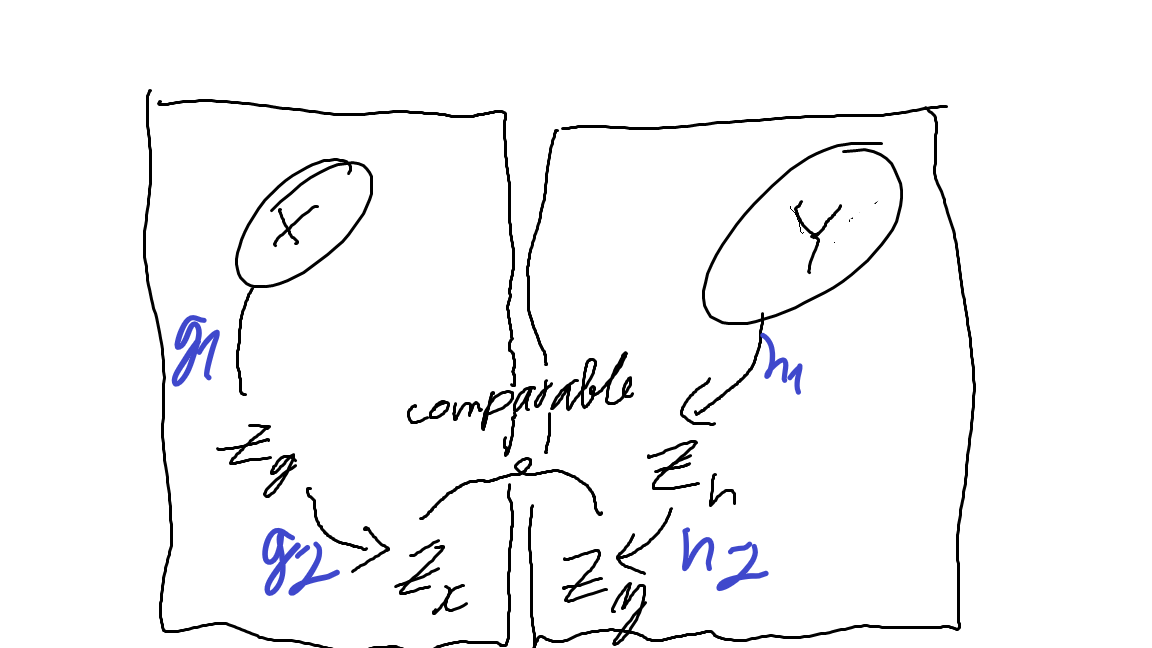
\includegraphics[width=12cm]{Untitled.png}\\

\centerline{\textbf{\small{sketch of a unified framework in machine learning}}}\\

How it works: Unlike human, a machine does not possess the ability to differentiate between things in a high-dimension space. In order for it to rate its performance, the information must be strip down to a lower dimension space, called "\textbf{embeddings}".\\

\hspace{1cm}The 'X' and 'Y' spaces represents the information that we want the machine to choose and extract; we can think of this as a \textbf{vector space}. Each vector is an attribute, called a \textbf{basis feature}, that a computer can extract from. Since the amount of vectors in the space can be enormous, and the capacity of a machine is by contrast limited, it must only choose some of the vectors available that we need.

\hspace{1cm}For example: we want the a machine to predict the taste of an ice-cream. To do so, we need it to pick out the color, the smell,... we don't need it to figure out what type of holder is holding the ice-cream, nor what type of person is holding the ice-cream.\\

In the above example, the X space would be the information about the ice-cream and the Y space would include words from a dictionary. 

The way we can extract the necessary information (color, smell,...) and words (sweet, bitter, strawberry, crunchy...) is by using some \textbf{basis function}. Each basis function corresponds to a specific type of information, e.g., color. \textbf{$g_1, g_2, h_1, h_2$} in the sketch are a collection of these basis functions. These produce a \textbf{coordinate vector Z} containing the picked-out information in both the X and Y vector space.

\section{Principal Component Analysis}

This is the simplest way we can reduce our high-dimensional vector space to a lower one. From our initial vector space, we can use this method to reduce it to the coordinate vector $Z_g$ and $Z_n$ in our sketch

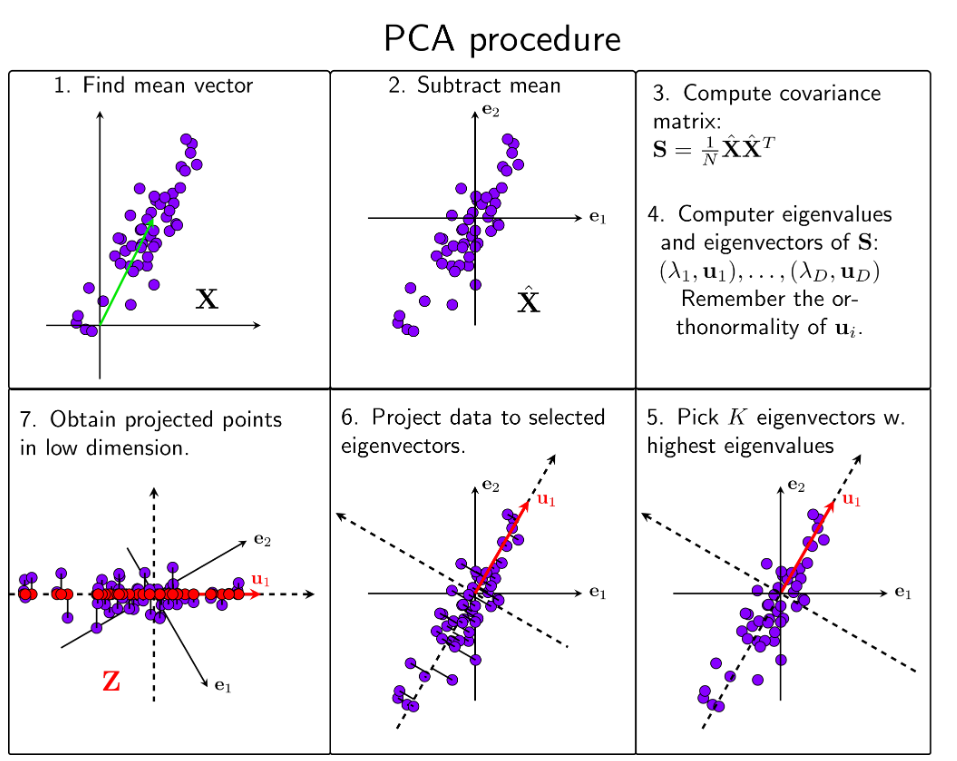
\includegraphics[width=12cm]{Capture.PNG}\\

After this step, if data from $Z_g$ and $Z_n$ can be expressed in the same vector space, we can compare their performance through either:
\begin{itemize}
  \item Calculating the Inner product 
  \item Calculating its distance between reality and machine-produced (e.g., real flavour to the flavour that the code gives).
  \item Many other methods depending on the type of data like Cross-entropy...
\end{itemize}

Else, we move on to the next step, which is to strip it down to an even lower dimension space.

\section{Linear regression}

This is a method used for specific types of information in statistics.

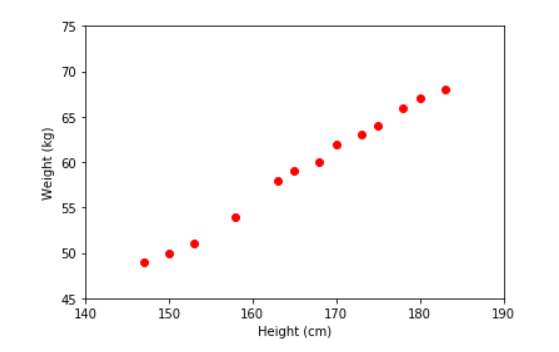
\includegraphics[width=12cm]{Capture2.PNG}\\

\centerline{\textbf{\small{graph of height compare to weight of 13 people}}}\\

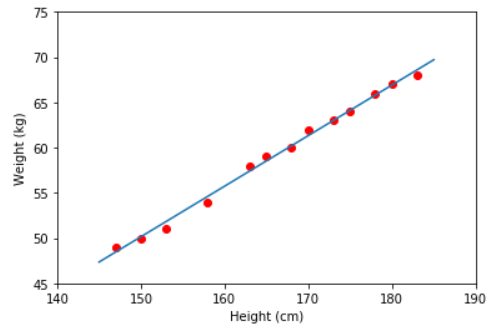
\includegraphics[width=12cm]{Capture3.PNG}\\

\centerline{\textbf{\small{Using linear regression to compute the line best fit}}}\\

This is one of the method that can be used to find the optimal functions for the next step after \textbf{PCA}, after which, it is stripped down to its simplest components and can be compared








\end{document}




